\subsection{Slicing and kick-off}
  Another small section is the \textit{'kick-off'}, usually a single meeting where the team gets together and discusses the tickets that makeup
  the project as a whole. 

  \begin{figure}[H]
    \centering
    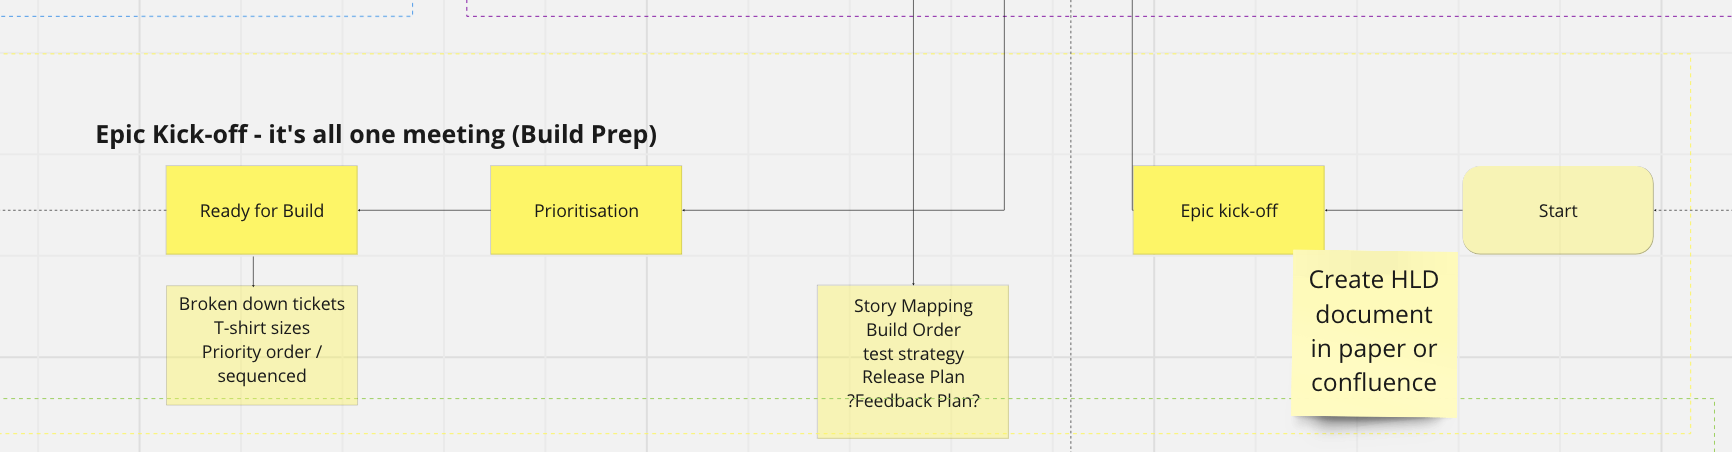
\includegraphics[width=8cm]{assets/workflow/kickoff.png}
    \caption{Kick-off stage of our ways of working.}
    \label{fig:workflowKickOff}
  \end{figure}

  Ideally this work has already been broken down into tasks. This is where the spike really helps, instead of guessing we are able to better understand 
  the work that needs doing and create tasks accordingly (Hashimi, Abduldaem, Gravell, 2022). The following diagram shows the initial breakdown of 
  tasks/tickets that were created for the project.

  \begin{figure}[H]
    \centering
    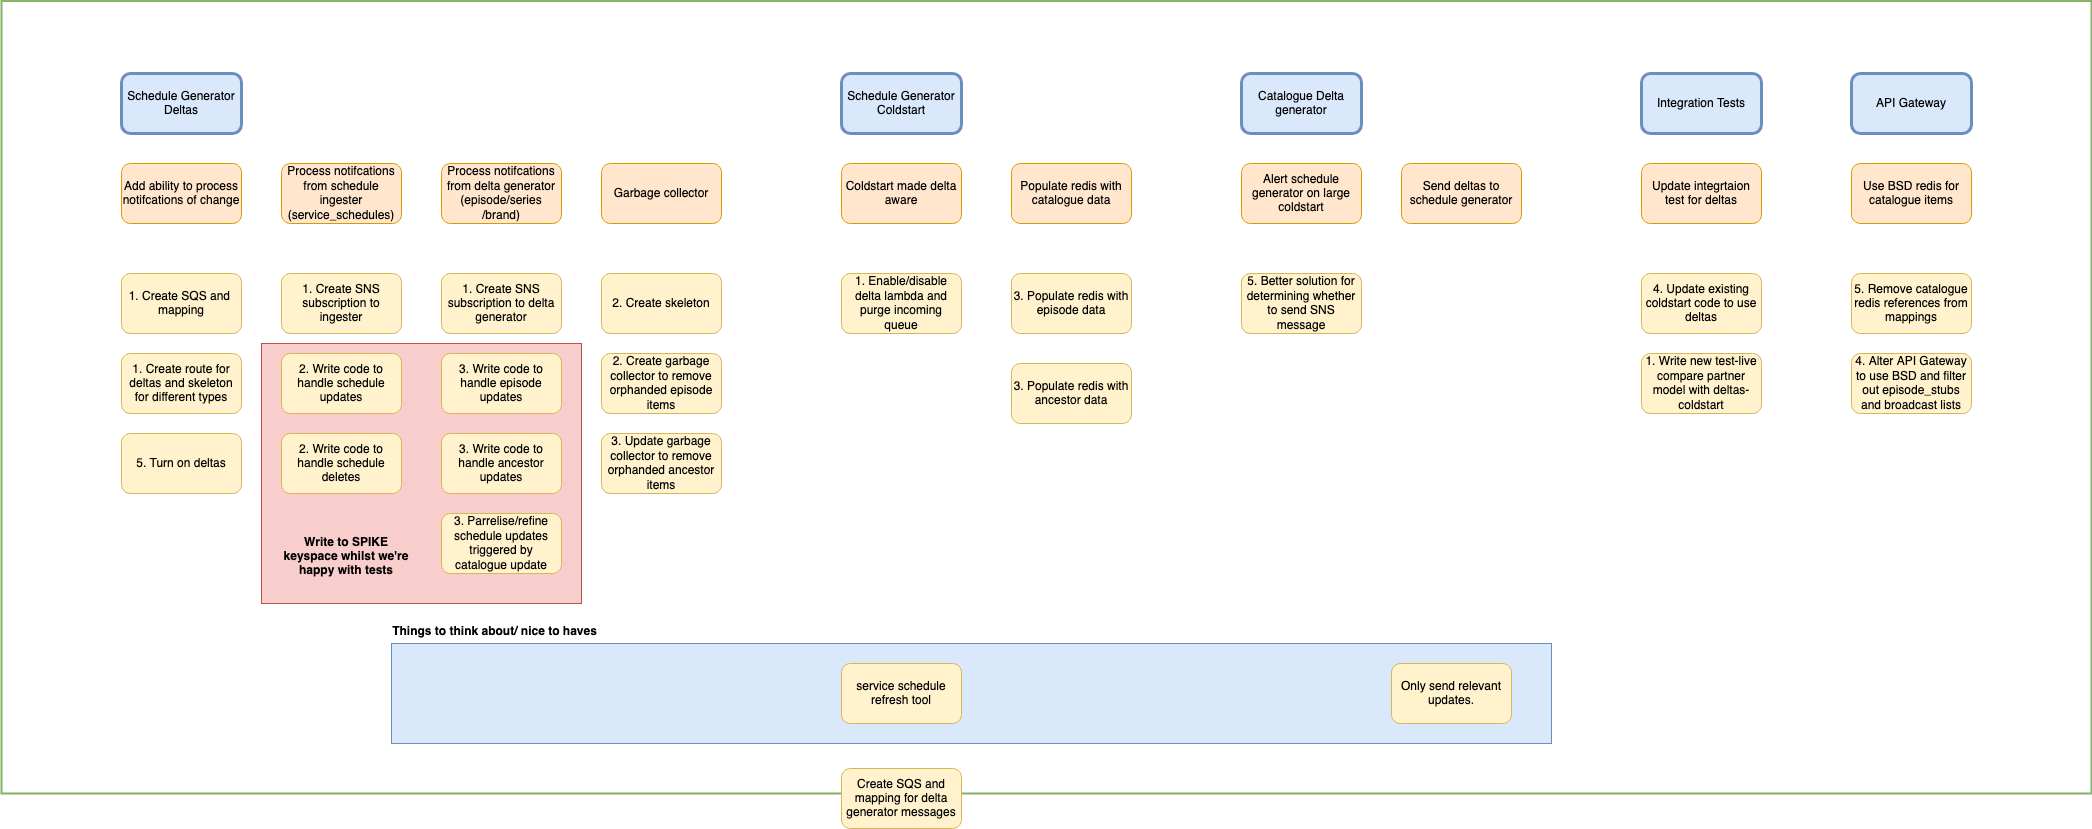
\includegraphics[width=14cm]{assets/schedulesSlicing.drawio.png}
    \caption{Pre-work slicing of work, organised vertically into components.}
    \label{fig:schedulesSlicing}
  \end{figure}

  A work breakdown structure (WBS) is a tool used to \textit{'break down deliverables into sub-deliverables to visualize projects'} (Raeburn, 2024) 
  and is typically broken down into 3 levels, parents, dependencies and sub-tasks, however it can consist of as any as a team wants. For the above I kept it 
  at 3 levels, going vertically, blue represents self-contained features/components, orange is a parent task to complete the feature and yellow is a 
  sub-task of the parent task. Numbers on the sub-tasks represent the initial prioritisation/ordering of the tasks into slices or feature sets.

  It's important to note that this is not the final list of tasks. Unknowns will always appear whilst developing the software and result in additional
  tasks being created. However the WBS helps refine the scope to what is needed (Burghate, 2018). As can be seen in the above figure there are 3 tasks that have 
  been moved to a \textit{'nice to have'} section, which have been deemed unnecessary for the projects initial completion.

  Another way to visualise these feature sets is using an Archimate implementation and migration diagram. This allows the modelling of work packages,
  gaps, deliverables, plateaus (stages) and events (The open group, 2016). The diagram on the next page shows the project mapped out using these elements, 
  documenting the deliverables for each feature set.

  \begin{figure}[H]
    \centering
    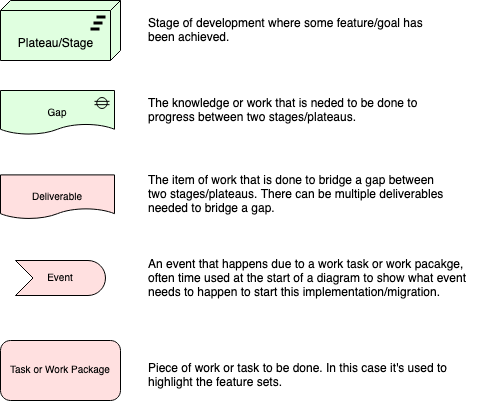
\includegraphics[width=6cm]{assets/migrationKey.drawio.png}
    \caption{Implementation and migration diagram components (The open group, 2016 and Jonkers et al, 2011).}
    \label{fig:migrationKey}
  \end{figure}

  \newpage

  \begin{landscape}
    \begin{figure}
      \centering
      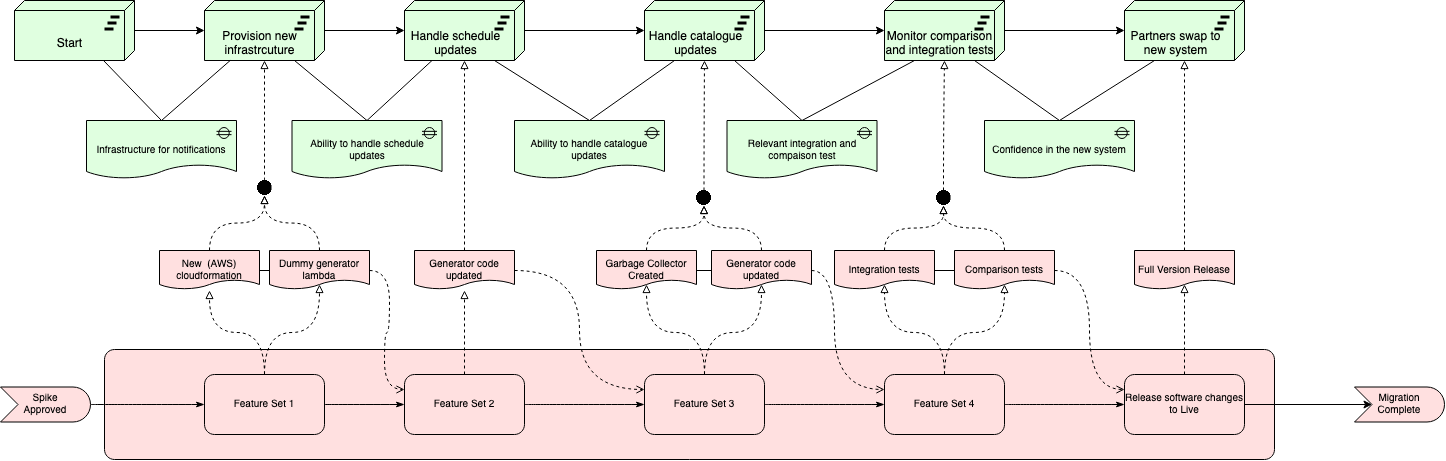
\includegraphics[width=20cm]{assets/migration.drawio.png}
      \caption{Figure showing Archimate implementation/migration diagram for project.}
      \label{fig:migration}
    \end{figure}
  \end{landscape}

\newpage